% !Mode:: "TeX:UTF-8"
\documentclass{article}

%%%%%%%%------------------------------------------------------------------------
%%%% 日常所用宏包

%% 控制页边距
% 如果是beamer文档类, 则不用geometry
\makeatletter
\@ifclassloaded{beamer}{}{\usepackage[top=2.5cm, bottom=2.5cm, left=2.5cm, right=2.5cm]{geometry}}
\makeatother

%% 控制项目列表
\usepackage{enumerate}

%% 多栏显示
\usepackage{multicol}

%% 算法环境
\usepackage{algorithm}  
\usepackage{algorithmic} 
\usepackage{float} 

%% 网址引用
\usepackage{url}

%% 控制矩阵行距
\renewcommand\arraystretch{1.4}

%% hyperref宏包,生成可定位点击的超链接,并且会生成pdf书签
\makeatletter
\@ifclassloaded{beamer}{
\usepackage{hyperref}
\usepackage{ragged2e} % 对齐
}{
\usepackage[%
    pdfstartview=FitH,%
    CJKbookmarks=true,%
    bookmarks=true,%
    bookmarksnumbered=true,%
    bookmarksopen=true,%
    colorlinks=true,%
    citecolor=blue,%
    linkcolor=blue,%
    anchorcolor=green,%
    urlcolor=blue%
]{hyperref}
}
\makeatother



\makeatletter % 如果是 beamer 不需要下面两个包
\@ifclassloaded{beamer}{
\mode<presentation>
{
} 
}{
%% 控制标题
\usepackage{titlesec}
%% 控制目录
\usepackage{titletoc}
}
\makeatother

%% 控制表格样式
\usepackage{booktabs}

%% 控制字体大小
\usepackage{type1cm}

%% 首行缩进,用\noindent取消某段缩进
\usepackage{indentfirst}

%% 支持彩色文本、底色、文本框等
\usepackage{color,xcolor}

%% AMS LaTeX宏包: http://zzg34b.w3.c361.com/package/maths.htm#amssymb
\usepackage{amsmath,amssymb}
%% 多个图形并排
\usepackage{subfig}
%%%% 基本插图方法
%% 图形宏包
\usepackage{graphicx}
\newcommand{\red}[1]{\textcolor{red}{#1}}
\newcommand{\blue}[1]{\structure{#1}}
\newcommand{\brown}[1]{\textcolor{brown}{#1}}
\newcommand{\green}[1]{\textcolor{green}{#1}}


%%%% 基本插图方法结束

%%%% pgf/tikz绘图宏包设置
\usepackage{pgf,tikz}
\usetikzlibrary{shapes,automata,snakes,backgrounds,arrows}
\usetikzlibrary{mindmap}
%% 可以直接在latex文档中使用graphviz/dot语言,
%% 也可以用dot2tex工具将dot文件转换成tex文件再include进来
%% \usepackage[shell,pgf,outputdir={docgraphs/}]{dot2texi}
%%%% pgf/tikz设置结束


\makeatletter % 如果是 beamer 不需要下面两个包
\@ifclassloaded{beamer}{

}{
%%%% fancyhdr设置页眉页脚
%% 页眉页脚宏包
\usepackage{fancyhdr}
%% 页眉页脚风格
\pagestyle{plain}
}

%% 有时会出现\headheight too small的warning
\setlength{\headheight}{15pt}

%% 清空当前页眉页脚的默认设置
%\fancyhf{}
%%%% fancyhdr设置结束


\makeatletter % 对 beamer 要重新设置
\@ifclassloaded{beamer}{

}{
%%%% 设置listings宏包用来粘贴源代码
%% 方便粘贴源代码,部分代码高亮功能
\usepackage{listings}

%% 设置listings宏包的一些全局样式
%% 参考http://hi.baidu.com/shawpinlee/blog/item/9ec431cbae28e41cbe09e6e4.html
\lstset{
showstringspaces=false,              %% 设定是否显示代码之间的空格符号
numbers=left,                        %% 在左边显示行号
numberstyle=\tiny,                   %% 设定行号字体的大小
basicstyle=\footnotesize,                    %% 设定字体大小\tiny, \small, \Large等等
keywordstyle=\color{blue!70}, commentstyle=\color{red!50!green!50!blue!50},
                                     %% 关键字高亮
frame=shadowbox,                     %% 给代码加框
rulesepcolor=\color{red!20!green!20!blue!20},
escapechar=`,                        %% 中文逃逸字符,用于中英混排
xleftmargin=2em,xrightmargin=2em, aboveskip=1em,
breaklines,                          %% 这条命令可以让LaTeX自动将长的代码行换行排版
extendedchars=false                  %% 这一条命令可以解决代码跨页时,章节标题,页眉等汉字不显示的问题
}}
\makeatother
%%%% listings宏包设置结束


%%%% 附录设置
\makeatletter % 对 beamer 要重新设置
\@ifclassloaded{beamer}{

}{
\usepackage[title,titletoc,header]{appendix}
}
\makeatother
%%%% 附录设置结束


%%%% 日常宏包设置结束
%%%%%%%%------------------------------------------------------------------------


%%%%%%%%------------------------------------------------------------------------
%%%% 英文字体设置结束
%% 这里可以加入自己的英文字体设置
%%%%%%%%------------------------------------------------------------------------

%%%%%%%%------------------------------------------------------------------------
%%%% 设置常用字体字号,与MS Word相对应

%% 一号, 1.4倍行距
\newcommand{\yihao}{\fontsize{26pt}{36pt}\selectfont}
%% 二号, 1.25倍行距
\newcommand{\erhao}{\fontsize{22pt}{28pt}\selectfont}
%% 小二, 单倍行距
\newcommand{\xiaoer}{\fontsize{18pt}{18pt}\selectfont}
%% 三号, 1.5倍行距
\newcommand{\sanhao}{\fontsize{16pt}{24pt}\selectfont}
%% 小三, 1.5倍行距
\newcommand{\xiaosan}{\fontsize{15pt}{22pt}\selectfont}
%% 四号, 1.5倍行距
\newcommand{\sihao}{\fontsize{14pt}{21pt}\selectfont}
%% 半四, 1.5倍行距
\newcommand{\bansi}{\fontsize{13pt}{19.5pt}\selectfont}
%% 小四, 1.5倍行距
\newcommand{\xiaosi}{\fontsize{12pt}{18pt}\selectfont}
%% 大五, 单倍行距
\newcommand{\dawu}{\fontsize{11pt}{11pt}\selectfont}
%% 五号, 单倍行距
\newcommand{\wuhao}{\fontsize{10.5pt}{10.5pt}\selectfont}
%%%%%%%%------------------------------------------------------------------------


%% 设定段间距
\setlength{\parskip}{0.5\baselineskip}

%% 设定行距
\linespread{1}


%% 设定正文字体大小
% \renewcommand{\normalsize}{\sihao}

%制作水印
\RequirePackage{draftcopy}
\draftcopyName{XTUMESH}{100}
\draftcopySetGrey{0.90}
\draftcopyPageTransform{40 rotate}
\draftcopyPageX{350}
\draftcopyPageY{80}

%%%% 个性设置结束
%%%%%%%%------------------------------------------------------------------------


%%%%%%%%------------------------------------------------------------------------
%%%% bibtex设置

%% 设定参考文献显示风格
% 下面是几种常见的样式
% * plain: 按字母的顺序排列,比较次序为作者、年度和标题
% * unsrt: 样式同plain,只是按照引用的先后排序
% * alpha: 用作者名首字母+年份后两位作标号,以字母顺序排序
% * abbrv: 类似plain,将月份全拼改为缩写,更显紧凑
% * apalike: 美国心理学学会期刊样式, 引用样式 [Tailper and Zang, 2006]

\makeatletter
\@ifclassloaded{beamer}{
\bibliographystyle{apalike}
}{
\bibliographystyle{unsrt}
}
\makeatother


%%%% bibtex设置结束
%%%%%%%%------------------------------------------------------------------------

%%%%%%%%------------------------------------------------------------------------
%%%% xeCJK相关宏包

\usepackage{xltxtra,fontspec,xunicode}
\usepackage[slantfont, boldfont]{xeCJK} 

%% 针对中文进行断行
\XeTeXlinebreaklocale "zh"             

%% 给予TeX断行一定自由度
\XeTeXlinebreakskip = 0pt plus 1pt minus 0.1pt

%%%% xeCJK设置结束                                       
%%%%%%%%------------------------------------------------------------------------

%%%%%%%%------------------------------------------------------------------------
%%%% xeCJK字体设置

%% 设置中文标点样式,支持quanjiao、banjiao、kaiming等多种方式
\punctstyle{kaiming}                                        
                                                     
%% 设置缺省中文字体
\setCJKmainfont[BoldFont={Adobe Heiti Std}, ItalicFont={Adobe Kaiti Std}]{Adobe Song Std}   
%% 设置中文无衬线字体
\setCJKsansfont[BoldFont={Adobe Heiti Std}]{Adobe Kaiti Std}  
%% 设置等宽字体
\setCJKmonofont{Adobe Heiti Std}                            

%% 英文衬线字体
\setmainfont{DejaVu Serif}                                  
%% 英文等宽字体
\setmonofont{DejaVu Sans Mono}                              
%% 英文无衬线字体
\setsansfont{DejaVu Sans}                                   

%% 定义新字体
\setCJKfamilyfont{song}{Adobe Song Std}                     
\setCJKfamilyfont{kai}{Adobe Kaiti Std}
\setCJKfamilyfont{hei}{Adobe Heiti Std}
\setCJKfamilyfont{fangsong}{Adobe Fangsong Std}
\setCJKfamilyfont{lisu}{LiSu}
\setCJKfamilyfont{youyuan}{YouYuan}

%% 自定义宋体
\newcommand{\song}{\CJKfamily{song}}                       
%% 自定义楷体
\newcommand{\kai}{\CJKfamily{kai}}                         
%% 自定义黑体
\newcommand{\hei}{\CJKfamily{hei}}                         
%% 自定义仿宋体
\newcommand{\fangsong}{\CJKfamily{fangsong}}               
%% 自定义隶书
\newcommand{\lisu}{\CJKfamily{lisu}}                       
%% 自定义幼圆
\newcommand{\youyuan}{\CJKfamily{youyuan}}                 

%%%% xeCJK字体设置结束
%%%%%%%%------------------------------------------------------------------------

%%%%%%%%------------------------------------------------------------------------
%%%% 一些关于中文文档的重定义
\newcommand{\chntoday}{\number\year\,年\,\number\month\,月\,\number\day\,日}
%% 数学公式定理的重定义

%% 中文破折号,据说来自清华模板
\newcommand{\pozhehao}{\kern0.3ex\rule[0.8ex]{2em}{0.1ex}\kern0.3ex}

\newtheorem{example}{例}                                   
\newtheorem{theorem}{定理}[section]                         
\newtheorem{definition}{定义}
\newtheorem{axiom}{公理}
\newtheorem{property}{性质}
\newtheorem{proposition}{命题}
\newtheorem{lemma}{引理}
\newtheorem{corollary}{推论}
\newtheorem{remark}{注解}
\newtheorem{condition}{条件}
\newtheorem{conclusion}{结论}
\newtheorem{assumption}{假设}

\makeatletter %
\@ifclassloaded{beamer}{

}{
%% 章节等名称重定义
\renewcommand{\contentsname}{目录}     
\renewcommand{\indexname}{索引}
\renewcommand{\listfigurename}{插图目录}
\renewcommand{\listtablename}{表格目录}
\renewcommand{\appendixname}{附录}
\renewcommand{\appendixpagename}{附录}
\renewcommand{\appendixtocname}{附录}
%% 设置chapter、section与subsection的格式
\titleformat{\chapter}{\centering\huge}{第\thechapter{}章}{1em}{\textbf}
\titleformat{\section}{\centering\sihao}{\thesection}{1em}{\textbf}
\titleformat{\subsection}{\xiaosi}{\thesubsection}{1em}{\textbf}
\titleformat{\subsubsection}{\xiaosi}{\thesubsubsection}{1em}{\textbf}

\@ifclassloaded{book}{

}{
\renewcommand{\abstractname}{摘要}
}
}
\makeatother

\renewcommand{\figurename}{图}
\renewcommand{\tablename}{表}

\makeatletter
\@ifclassloaded{book}{
\renewcommand{\bibname}{参考文献}
}{
\renewcommand{\refname}{参考文献} 
}
\makeatother

\floatname{algorithm}{算法}
\renewcommand{\algorithmicrequire}{\textbf{输入:}}
\renewcommand{\algorithmicensure}{\textbf{输出:}}

%%%% 中文重定义结束
%%%%%%%%------------------------------------------------------------------------

\setCJKmainfont{STKaiti} % 如果请替换为本地系统有的字体
%中文断行
\XeTeXlinebreaklocale "zh"
\XeTeXlinebreakskip = 0pt plus 1pt minus 0.1pt
\begin{document}
\title{重心坐标与基函数}
%\date{\today}
\maketitle
%\tableofcontents
%\newpage
\section{重心坐标}
重心坐标是构造基函数的基础,所以首先引入重心坐标。

数学中,重心坐标是由单形(如三角形或四面体等)顶点定义的坐标。经典的重心坐标是一种定义在“多边形”上的坐标,而不局限于具体的坐标系。“多边形”内的点由“多边形”各顶点线性表出,组合系数便是重心坐标。下面定义重心坐标,以平面上的多边形为例。

令 $P$ 是一个平面上的 $n$ 边形,其顶点记为 $\lbrace X_i\rbrace_{i=0,\cdots,n}$,~$n\ge 2$,且以逆时针顺序标记。对任意的 $X\in P$,定义函数 $\lambda _i(x):P\longrightarrow R,~i=0,\cdots,n$.若

$$
X=\sum_{i=0}^n \lambda _i(X)X_i,~\sum_{i=0}^n\lambda _i(X)\equiv 1.
$$
则称 $\lambda _i(X)$ 为齐次坐标,此外,若 $\lambda _i(X)\ge 0,~i=0,\cdots,n$,则称 $\lambda _i(X)$ 为重心坐标。显然可以将上式看作一个以 $\lambda _i(X)$ 为未知量,$X$ 和 $X_i$ 为已知量的非齐次线性方程组,即重心坐标是方程组的非负解。当 $n=2$ 时,
$$
\begin{cases}
\lambda _0(X)x_0+\lambda _1(X)x_1+\lambda _2(X)x_2=x,\\
\lambda _0(X)y_0+\lambda _1(X)y_1+\lambda _2(X)y_2=y,\\
\lambda _0(X)+\lambda _1(X)+\lambda _2(X)=1.
\end{cases}
$$
即
$$
\begin{bmatrix}
x_0 & x_1 & x_2\\
y_0 & y_1 & y_2\\
1 & 1 & 1\\
\end{bmatrix}
\begin{bmatrix}
\lambda _0(X)\\
\lambda _1(X)\\
\lambda _2(X)\\
\end{bmatrix}=\begin{bmatrix}
x\\
y\\
1\\
\end{bmatrix}.
$$
由 $\begin{bmatrix}
x_0 & x_1 & x_2\\
y_0 & y_1 & y_2\\
1 & 1 & 1\\
\end{bmatrix}$ 的非奇异可知,$\lambda _0(X)$,$\lambda _1(X)$,$\lambda _2(X)$ 存在唯一。

重心坐标的几何意义:

\begin{figure}[H]
\centering
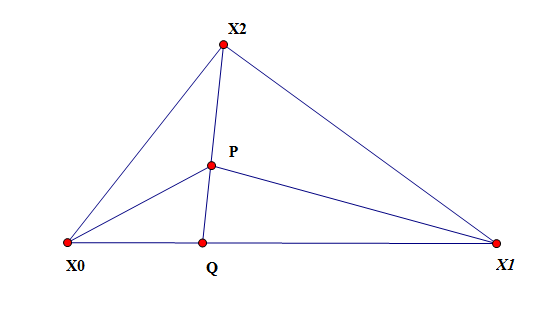
\includegraphics[scale=0.7]{./figures/2.png}
\caption{}
\end{figure}

任取 $P\in \triangle_{X_0 X_1 X_2}$,延长 $X_2 P$ 使之与 $X_0 X_1$ 相交于点 $Q$,则
$$
\lambda _2=\frac {PQ}{X_2 P}=\frac{S_{\triangle PX_0 X_1}}{S_{\triangle X_0 X_1 X_2}}.
$$

类似的可以定义一维,高维的重心坐标,定义高维重心坐标时,顶点要遵循右手法则。

\section{单纯形上的基函数}
区间 $[x_0,x_1]$ 上 $p$ 次拉格朗日基函数的构造

首先构造一维区间 $[x_0,x_1]$ 上的重心坐标,
$$
\begin{cases}
\lambda _0(x)x_0+\lambda _1(x)x_1=x,\\
\lambda _0(x)+\lambda _1(x)=1.
\end{cases}
$$
则,
$$
\begin{bmatrix}
x_0 & x_1\\
1 & 1\\
\end{bmatrix}
\begin{bmatrix}
\lambda _0(x)\\
\lambda _1(x)\\
\end{bmatrix}=\begin{bmatrix}
x\\
1\\
\end{bmatrix},
$$
因此,
$$
\lambda _0(x)=\frac{\begin{vmatrix}
x & x_1 \\
1 & 1 \\
\end{vmatrix}}{\begin{vmatrix}
x_0 & x_1 \\
1 & 1 \\
\end{vmatrix}}=\frac{x-x_1}{x_0-x_1}=\frac{x_1-x_0}{x_1-x_0},
\quad\lambda _1(x)=\frac{\begin{vmatrix}
x_0 & x \\
1 & 1
\end{vmatrix}}{\begin{vmatrix}
x_0 & x_1 \\
1 & 1
\end{vmatrix}}=\frac{x_0-x}{x_0-x_1}=\frac{x-x_0}{x_1-x_0}.
$$
$\forall x\in [x_0,x_1]$,则 $\lambda _0(x)\ge 0$,$\lambda _1(x)\ge 0$.并且
$$
\begin{cases}
\lambda _0 (x_0)=1,\lambda _0 (x_1)=0,\\
\lambda _1 (x_0)=0,\lambda _1 (x_1)=1.\\
\end{cases}
$$
易知, $\lambda_0, \lambda_1$ 都是关于 $x$ 的线性函数(这里指一次函数)。

重心坐标关于 $x$ 的导数为:
$$
\frac{\mathrm d \lambda_0}{\mathrm dx} = -\frac{1}{x_1 - x_0},\quad 
\frac{\mathrm d \lambda_1}{\mathrm dx} = \frac{1}{x_1 - x_0}.
$$
区间 $[x_0, x_1]$ 上的 $p\geq 1$ 次基函数共有 
$n_{dof} = p+1$ 个,

其插值基函数的计算公式如下:
$$
\phi_{m,n} = \frac{p^p}{m!n!}\prod_{l_0 = 0}^{m - 1}
(\lambda_0 - \frac{l_0}{p}) \prod_{l_1 = 0}^{n-1}(\lambda_1 -
\frac{l_1}{p}).
$$
其中 $m\geq 0$, $n\geq 0$, 且 $m+n=p$,即 $\phi_{m,n}$ 是一个 $m+n=p$ 次多项式。

由 $\frac{x_1 - x}{x_1 - x_0}=\frac{l_0}{p}$ 得到
$$
x=x_1-\frac{l_0}{p} (x_1 - x_0)=(1-\frac{l_0}{p})x_1 + \frac{l_0}{p} x_0.
$$
因为 $(1-\frac{l_0}{p}) + \frac{l_0}{p} =1$,故 $x\in [x_0,x_1].$

由 $\frac{x - x_0}{x_1 - x_0}=\frac{l_1}{p}$ 得到
$$
x=x_0+\frac{l_1}{p} (x_1 - x_0)=\frac{l_1}{p})x_1 + (1-\frac{l_1}{p})x_0.
$$
因为 $(1-\frac{l_1}{p}) + \frac{l_1}{p} = 1$,故 $x\in [x_0,x_1].$

因此插值基函数过节点 $x_1,\frac{(p-1)x_1 + x_0}{p},\frac{(p-2)x_1 + 2x_0}{p},\frac{(p-3)x_1 + 3x_0}{p},\cdots,x_0$,即把区间 $[x_0,x_1]$ 均匀等分,步长为 $\frac{(x_1-x_0)}{p}$.

这个 $p$ 次插值基函数实际上就是这种形式的
$$
l_k(x)=\frac{(x-x_0)\cdots(x-x_{k-1})(x-x_{k+1})\cdots(x - x_p)}{(x_k-x_0)\cdots(x_k-x_{k-1})(x_k-x_{k+1})\cdots(x_k-x_p)}
$$
拉格朗日插值基函数。

$p$ 次基函数的面向数组的计算
构造向量:
$$
P = ( \frac{1}{0!},  \frac{1}{1!}, \frac{1}{2!}, \cdots, \frac{1}{p!})
$$

构造矩阵:
$$
A :=                                                                            
\begin{pmatrix}  
1  &  1  \\
\lambda_0 & \lambda_1\\                                             
\lambda_0 - \frac{1}{p} & \lambda_1 - \frac{1}{p}\\   
\vdots & \vdots \\                                                     
\lambda_0 - \frac{p - 1}{p} & \lambda_1 - \frac{p - 1}{p}
\end{pmatrix}                                                                   
$$ 
对 $A$ 的每一列做累乘运算, 并左乘由 $P$ 形成的对角矩阵, 得矩阵:

$$
B = \mathrm{diag}(P)
\begin{pmatrix}
1 & 1\\
\lambda_0 & \lambda_1\\
\prod_{l=0}^{1}(\lambda_0 - \frac{l}{p}) & \prod_{l=0}^{1}(\lambda_1 - \frac{l}{p})\\
\vdots & \vdots \\
\prod_{l=0}^{p-1}(\lambda_0 - \frac{l}{p}) & \prod_{l=0}^{p-1}(\lambda_1 - \frac{l}{p}) 
\end{pmatrix}
$$

易知, 只需从 $B$ 的每一列中各选择一项相乘(要求二项次数之和为 $p$), 再乘以 $p^p$ 即可得到相应的基函数, 其中取法共有 

$$
n_{dof} = {p+1}
$$

构造指标矩阵:

$$
I = \begin{pmatrix}
p  & 0 \\ p-1 & 1 \\ \vdots & \vdots \\ 0 & p 
\end{pmatrix}
$$
由$I$可知一共有$\begin{matrix} p+1 \\ \overbrace{ 1+1+\cdots+1 }
\end{matrix}$种选择。

\section{三角形单元}
下面考虑二维三角形单元的重心坐标。

给定三角形单元 $\tau$, 其三个顶点 $\mathbf x_0 :=(x_0,y_0)$, $\mathbf x_1 :=(x_1,y_1)$ 和 $\mathbf x_2 :=(x_2,y_2)$ 逆时针排列, 且不在同一条直线上, 那么向量 $\overrightarrow{\mathbf x_0\mathbf x_1}$ 和 $\overrightarrow{\mathbf x_0\mathbf x_2}$ 是线性无关的. 这等价于矩阵

$$
A = 
\begin{pmatrix}
x_0 & x_1 & x_2 \\
y_0 & y_1 & y_2 \\
1   & 1   & 1 
\end{pmatrix}
$$

非奇异. 
又 $|A|\ne 0$,故任给一点 $\mathbf{x}:=(x,y)\in\tau$,下面的线性方程组

$$
A 
\begin{pmatrix}
\lambda_0 \\
\lambda_1\\
\lambda_2  
\end{pmatrix}
=\begin{pmatrix}
x \\
y\\
1  
\end{pmatrix}
$$

有唯一的一组解 $\lambda_0,\lambda_1,\lambda_2$. 
因此对任意二维点 $\mathbf{x}\in\tau$, 有
$$
\begin{cases}
\lambda _0 x_0+\lambda _1 x_1+\lambda _2 x_2=x,\\
\lambda _0 y_0+\lambda _1 y_1+\lambda _2 y_2=y,\\
\lambda _0+ \lambda _1 +\lambda _2 =1.
\end{cases}
$$
故$\lambda _0 (x_0,y_0)+\lambda _1 (x_1,y_1)+\lambda _2 (x_2,y_2)=(x,y)$,
$$
\mathbf{x}=\lambda_0(\mathbf{x})\mathbf{x}_0 + \lambda_1(\mathbf{x})\mathbf{x}_1 + \lambda_2(\mathbf{x})\mathbf{x}_2 
\text{ 且 } \lambda_0(\mathbf{x}) + \lambda_1(\mathbf{x}) + \lambda_2(\mathbf{x}) = 1. 
$$

$\lambda_0,\lambda_1,\lambda_2$ 称为点 $\mathbf{x}$ 关于点 $\mathbf{x}_0,\mathbf{x}_1$ 和$\mathbf{x}_2$ 的重心坐标. 

易知, $\lambda_0, \lambda_1, \lambda_2$ 都是关于 $\mathbf x$ 的线性函数, 且有

\begin{eqnarray*}
\lambda_0(\mathbf x_0) = 1,\quad & \lambda_0(\mathbf x_1) = 0,\quad& \lambda_0(\mathbf x_2) = 0\\
\lambda_1(\mathbf x_0) = 0,\quad & \lambda_1(\mathbf x_1) = 1,\quad& \lambda_1(\mathbf x_2) = 0\\
\lambda_2(\mathbf x_0) = 0,\quad & \lambda_2(\mathbf x_1) = 0,\quad & \lambda_2(\mathbf x_2) = 1\\
\end{eqnarray*}

\begin{figure}[H]
\centering
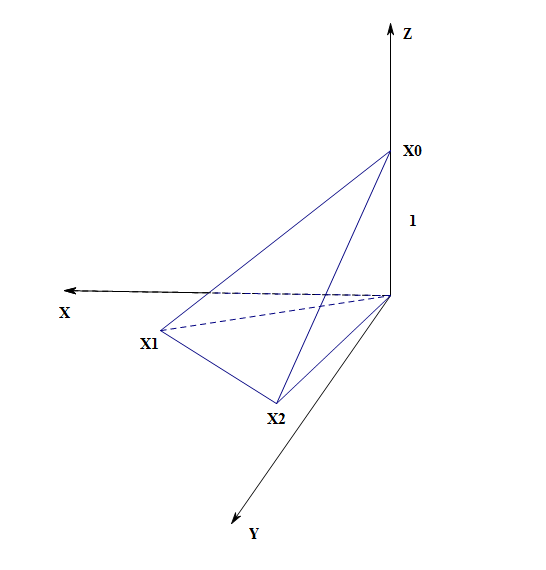
\includegraphics[scale=0.7]{./figures/3.png}
\caption{}
\end{figure}

也可以通过下面的方式计算重心坐标。

设 $\lambda_0 (x,y)=ax+by+c$,则
$$
\begin{cases}
\lambda _0 (x_0,y_0)=ax_0+by_0+c=1,\\
\lambda _0 (x_1,y_1)=ax_1+by_1+c=0,\\
\lambda _0 (x_2,y_2)=ax_2+by_2+c=0.\\
\end{cases}
$$
从而可以求出 $a$,$b$,$c$,进而求出 $\lambda _0$.同理可得 $\lambda _1$,$\lambda _2$.

为了考虑变化率的大小和方向,引入梯度。梯度的大小是变化率最大的值,梯度的方向是变化率最大的方向。

$\lambda_0, \lambda_1, \lambda_2$ 关于 $\mathbf x$ 的梯度分别为:

$$
\begin{aligned}
\nabla\lambda_0 = \frac{1}{2|\tau|}(\mathbf x_2 - \mathbf x_1)W\\
\nabla\lambda_1 = \frac{1}{2|\tau|}(\mathbf x_0 - \mathbf x_2)W\\
\nabla\lambda_2 = \frac{1}{2|\tau|}(\mathbf x_1 - \mathbf x_0)W\\
\end{aligned}
$$

其中 

$$
W = \begin{pmatrix}
0 & 1\\ -1 & 0 
\end{pmatrix}
$$
三角形单元上的 $p$ 次基函数公式

给定三角形单元上的一个重心坐标 $(\lambda_0, \lambda_1, \lambda_2)$, 所有 $p\geq 1$ 次基函数的计算公式如下:

$$
\phi_{m,n,k} = \frac{p^p}{m!n!k!}\prod_{l_0 = 0}^{m - 1}
(\lambda_0 - \frac{l_0}{p}) \prod_{l_1 = 0}^{n-1}(\lambda_1 -
\frac{l_1}{p}) \prod_{l_2=0}^{k-1}(\lambda_2 - \frac{l_2}{p}).
$$

其中 $ m\geq 0$, $n\geq 0$, $ k \geq 0$, 且 $m+n+k=p$.

因为$\lambda_0 (x_2,y_2) = 0,\lambda_1 (x_0,y_0) = 0,\lambda_2 (x_1,y_1) = 0$,因此插值基函数一定过节点$(x_0,y_0),(x_1,y_1),(x_2,y_2).$
因为$\lambda_0 (\frac{x_1+x_2}{2}) = 0,\lambda_1 (\frac{x_0+x_2}{2}) = 0,\lambda_2 (\frac{x_0+x_1}{2}) = 0$,因此插值基函数过节点$(\frac{x_1+x_2}{2},\frac{y_1+y_2}{2}),(\frac{x_0+x_2}{2},\frac{y_0+y_2}{2}),(\frac{x_0+x_1}{2},\frac{y_0+y_1}{2})$

$\cdots$
即把三角形单元均匀剖分。




















\newpage
\nocite{*}
\bibliography{ref}
\end{document}

